%%%%%%%% ICML 2018 EXAMPLE LATEX SUBMISSION FILE %%%%%%%%%%%%%%%%%

\documentclass{article}

% Recommended, but optional, packages for figures and better typesetting:
\usepackage{microtype}
\usepackage{graphicx}
\usepackage{subfigure}
\usepackage{amsmath}
\usepackage{booktabs} % for professional tables
% hyperref makes hyperlinks in the resulting PDF.
% If your build breaks (sometimes temporarily if a hyperlink spans a page)
% please comment out the following usepackage line and replace
% \usepackage{icml2018} with \usepackage[nohyperref]{icml2018} above.
%\usepackage{hyperref}

% Attempt to make hyperref and algorithmic work together better:
\newcommand{\theHalgorithm}{\arabic{algorithm}}

% Use the following line for the initial blind version submitted for review:
\usepackage{icml2018}

% If accepted, instead use the following line for the camera-ready submission:
%\usepackage[accepted]{icml2018}

% The \icmltitle you define below is probably too long as a header.
% Therefore, a short form for the running title is supplied here:
\icmltitlerunning{A Network Model for Dynamic Textual Communications with Application to Government Email Corpora}

\begin{document}

\twocolumn[
\icmltitle{Suplementary Materials for ``A Network Model for Dynamic Textual Communications with Application to Government Email Corpora"}

% It is OKAY to include author information, even for blind
% submissions: the style file will automatically remove it for you
% unless you've provided the [accepted] option to the icml2018
% package.

% List of affiliations: The first argument should be a (short)
% identifier you will use later to specify author affiliations
% Academic affiliations should list Department, University, City, Region, Country
% Industry affiliations should list Company, City, Region, Country

% You can specify symbols, otherwise they are numbered in order.
% Ideally, you should not use this facility. Affiliations will be numbered
% in order of appearance and this is the preferred way.
%\icmlsetsymbol{equal}{*}

\begin{icmlauthorlist}
\icmlauthor{Bomin Kim}{to}
\icmlauthor{Aaron Schein}{goo}
\icmlauthor{Bruce Desmarais}{ed}
\icmlauthor{Hanna Wallach}{equal,to}
\end{icmlauthorlist}

\icmlaffiliation{to}{Department of Statistics, Pennsylvania State University, Pennsylvania, USA}
\icmlaffiliation{goo}{College of Information and Computer Sciences, University of Massachusetts Amherst, Massachusetts, USA}
\icmlaffiliation{ed}{Department of Political Science, Pennsylvania State University,Pennsylvania, USA}
\icmlaffiliation{equal}{Microsoft Research NYC, New York, USA}

\icmlcorrespondingauthor{Cieua Vvvvv}{c.vvvvv@googol.com}
\icmlcorrespondingauthor{Eee Pppp}{ep@eden.co.uk}

% You may provide any keywords that you
% find helpful for describing your paper; these are used to populate
% the "keywords" metadata in the PDF but will not be shown in the document
%\icmlkeywords{Machine Learning, ICML}

\vskip 0.3in
]

% this must go after the closing bracket ] following \twocolumn[ ...

% This command actually creates the footnote in the first column
% listing the affiliations and the copyright notice.
% The command takes one argument, which is text to display at the start of the footnote.
% The \icmlEqualContribution command is standard text for equal contribution.
% Remove it (just {}) if you do not need this facility.

%\printAffiliationsAndNotice{}  % leave blank if no need to mention equal contribution
\printAffiliationsAndNotice{\icmlEqualContribution} % otherwise use the standard text.

\section{Normalizing constant of Gibbs measure}\label{sec: non-empty Gibbs measure}
 	 The non-empty Gibbs measure defines the probability of author $a$ selecting the binary recipient vector $\boldsymbol{u}_{ad}$ as
 	 \begin{equation*} 
 	 	\begin{aligned}
 	 		& P(\boldsymbol{u}_{ad}| \delta, \boldsymbol{\lambda}_{ad} ) \\&= \frac{\exp\Big\{ \mbox{log}\big(\text{I}(\lVert \boldsymbol{u}_{ad} \rVert_1 > 0)\big) + \sum_{r \neq a} (\delta+\lambda_{adr})u_{adr} \Big\}}{Z(\delta,\boldsymbol{\lambda}_{ad})}.
 	 	\end{aligned}
 	 \end{equation*}
 	 
 	 To use this distribution efficiently, we derive a closed-form expression for $Z(\delta,\boldsymbol{\lambda}_{id})$ that does not require brute-force summation over the support of $\boldsymbol{u}_{ad}$ (\textit{i.e.} $\forall \boldsymbol{u}_{ad} \in [0,1]^A$). We recognize that if $\boldsymbol{u}_{ad}$ were drawn via independent Bernoulli distributions in which $P({u}_{adr}=1|\delta, \boldsymbol{\lambda}_{ad})$ was given by logit$(\delta+\lambda_{adr})$, then 
 	 \begin{equation*}
 	 	P(\boldsymbol{u}_{ad}|\delta, \boldsymbol{\lambda}_{ad}) \propto \exp\Big\{\sum_{r \neq a } (\delta+\lambda_{adr})u_{adr}\Big\}.  	 
 	 \end{equation*}
 	 This is straightforward to verify by looking at 
 	 \begin{equation*}
 	 	\begin{aligned}
 	 		&P(u_{adr}=1|\boldsymbol{u}_{ad[-r]}, \delta, \boldsymbol{\lambda}_{ad})
 	 		=\frac{ \exp{(\delta+\lambda_{adr})}}{\exp{(\delta+\lambda_{adr})} + 1}.\end{aligned}\end{equation*}
 	 We denote the logistic-Bernoulli normalizing constant as $Z^{l}(\delta,\boldsymbol{\lambda}_{ad})$, which is defined as 
 	 \begin{equation*}
 	 	Z^{l}(\delta,\boldsymbol{\lambda}_{ad})=\sum_{\boldsymbol{u}_{ad} \in [0,1]^{A}} \exp\Big\{\sum_{r\neq a} (\delta+\lambda_{adr})u_{adr}\Big\}.
 	 \end{equation*}
 	 Now, since 
 	 \begin{equation*}
 	 	\begin{aligned}
 	 		&\exp\Big\{ \mbox{log}\Big(\text{I}(\lVert \boldsymbol{u}_{ad} \rVert_1 > 0)\Big) + \sum_{r \neq a} (\delta+\lambda_{adr})u_{adr} \Big\}\\&= \exp\Big\{  \sum_{r \neq a} (\delta+\lambda_{adr})u_{adr} \Big\},
 	 	\end{aligned}
 	 \end{equation*}
 	 except when $\lVert \boldsymbol{u}_{ad} \rVert_1=0$, we note that 
 	 \begin{equation*}
 	 	\begin{aligned}
 	 		Z(\delta,\boldsymbol{\lambda}_{ad})& = Z^{l}(\delta,\boldsymbol{\lambda}_{ad}) -\exp\Big\{ \sum\limits_{\forall u_{adr}=0}(\delta+\lambda_{adr})u_{adr} \Big\}
 	 		\\& = Z^{l}(\delta,\lambda_{a}^{(d)}) -  1.
 	 	\end{aligned}
 	 \end{equation*}
 	 We can therefore derive a closed form expression for $Z(\delta,\boldsymbol{\lambda}_{ad})$ via a closed form expression for $Z^{l}(\delta,\boldsymbol{\lambda}_{ad})$. This can be done by looking at the probability of the zero vector under the logistic-Bernoulli model:
 	 \begin{equation*}
 	 	\begin{aligned}
 	 		&\frac{\exp\Big\{ \sum\limits_{\forall u_{adr}=0}(\delta+\lambda_{adr})u_{adr} \Big\}}{Z^{l}(\delta,\boldsymbol{\lambda}_{ad})}= \prod_{r \neq a}   \Big(1-\frac{ \exp{(\delta+\lambda_{adr})}}{\exp{(\delta+\lambda_{adr})} + 1}\Big).
 	 	\end{aligned}  
 	 \end{equation*}
 	 Then, we have 
 	 \begin{equation*}
 	 	\begin{aligned}
 	 		& \frac{1}{Z^{l}(\delta,\boldsymbol{\lambda}_{ad})} &= \prod\limits_{r \neq a}\frac{1}{ \exp(\delta+\lambda_{adr})+ 1}.
 	 	\end{aligned}  
 	 \end{equation*}
 	 Finally, the closed form expression for the normalizing constant under the non-empty Gibbs measure is  \begin{equation*}
 	 	\begin{aligned}Z(\delta,\boldsymbol{\lambda}_{ad}) = \prod_{r \neq a } \big(\mbox{exp}\{\delta+\lambda_{adr}\} + 1\big)-1.
 	 	\end{aligned}  
 	 \end{equation*}
 	 
\iffalse
 \section{Specification of Network Features}\label{sec:Specification of Network Features}
We provide the details on the specification of $\boldsymbol{x}_{adrc} = ({x}^1_{adrc}, {x}^2_{adrc}, {x}^3_{adrc})$ in Section 4.2. We first partitioned the interval $[t_d-16d, t_d)$ into $L=3$ sub-intervals with equal length in the log-scale, by setting the difference $\Delta_l$ = (6 hours) $\times  4^l$ for $l=1,2,3$. In other words, we define the intervals $I_d^l$ by 
 \begin{equation*}
 \footnotesize
 \begin{aligned}
 &[t_d-384h,t_d) \\&=[t_d-384h, t_d-96h) \cup [t_d-96h, t_d-24h)\cup [t_d-24h, t_d)
 \\&=I_d^{3}\cup  I_d^{2}\cup I_d^{1},
 \end{aligned}
 \end{equation*}
 where $I_{d}^{l} $ is the half-open interval $[t_d-\Delta_l, t_d-\Delta_{l-1})$. 
 
 Then, for each time interval $l=1,2,3$, the degree and dyadic statistics are defined as:
 \begin{itemize}
 	 	\footnotesize
 	\item [1.]  $\mbox{\textbf{outdegree}}^l_{id\cdot c}=\sum\limits_{d \in I_{d}^{l}}\pi_{dc}I\{i\rightarrow \forall j\}$
 	\item [2.] $\mbox{\textbf{indegree}}^l_{\cdot dj c}=\sum\limits_{d \in I_{d}^{l}}\pi_{dc}I\{\forall i \rightarrow j\}$	 	 	
 	\item [3.]  $\mbox{\textbf{send}}^l_{idjc}=\sum\limits_{d \in I_{d}^{l}}\pi_{dc} I\{i\rightarrow j\}$
 	\item [4.] $\mbox{\textbf{receive}}^l_{idjc}=\sum\limits_{d\in I_{d}^{l}}\pi_{dc} I\{j\rightarrow i\}$
 \end{itemize}
 \normalsize
 Next, we define four triadic statistics involving pairs of messages, which are analogous to 2-path statistics commonly used in the network science literature. While earlier works (Perry \& Wolfe, 2013) adapted full sets of triadic statistics for each combination of time intervals (e.g. $3 \times 3=9$), we maintain 3 intervals per each statistic, by defining $3 \times 3$ time windows and sum the combination-specific statistics based on the interval where the triads are closed (Refer to Figure 1). As a result, our interval-adjusted definitions of triadic effects become
 \begin{itemize}
 	\footnotesize
 	\item [5.] $\mbox{\textbf{2-send}}^l_{idjc}=\vspace{3mm}\\\sum\limits_{\substack{\max(l_1,l_2)= l} }\sum\limits_{\substack{h \neq i\\h \neq  j} }(\sum\limits_{d\in I_{d}^{l_1}}\pi_{dc} I\{i\rightarrow h\})(\sum\limits_{d\in I_{d}^{l_2}}\pi_{dc}I\{h\rightarrow j\})$\\
 	\item [6.] $\mbox{\textbf{2-receive}}^l_{idjc}=\vspace{3mm}\\\sum\limits_{\substack{\max(l_1,l_2)= l} }\sum\limits_{\substack{h \neq i\\h \neq  j} }(\sum\limits_{d \in I_{d}^{l_1}}\pi_{dc} I\{h\rightarrow i\})(\sum\limits_{d\in I_{d}^{l_2}}\pi_{dc} I\{j\rightarrow h\})$
 	\item [7.] $\mbox{\textbf{sibling}}^l_{idjc}=\vspace{3mm}\\\sum\limits_{\substack{\max(l_1,l_2)= l} }\sum\limits_{\substack{h \neq i\\h \neq  j} }(\sum\limits_{d\in I_{d}^{l_1}}\pi_{dc} I\{h\rightarrow i\}) (\sum\limits_{d\in I_{d}^{l_2}}\pi_{dc}I\{h\rightarrow j\})$
 	\item [8.] $\mbox{\textbf{cosibling}}^l_{idjc}=\vspace{3mm}\\\sum\limits_{\substack{\max(l_1,l_2)= l}}\sum\limits_{\substack{h \neq i\\h \neq  j} }(\sum\limits_{d \in I_{d}^{l_1}}\pi_{dc} I\{i\rightarrow h\})(\sum\limits_{d\in I_{d}^{l_2}}\pi_{dc}I\{j\rightarrow h\})$
 \end{itemize}
 where $l_1=1,2,3$ and $l_2=1,2,3$. 
 \begin{figure}[ht]
 	\centering
 	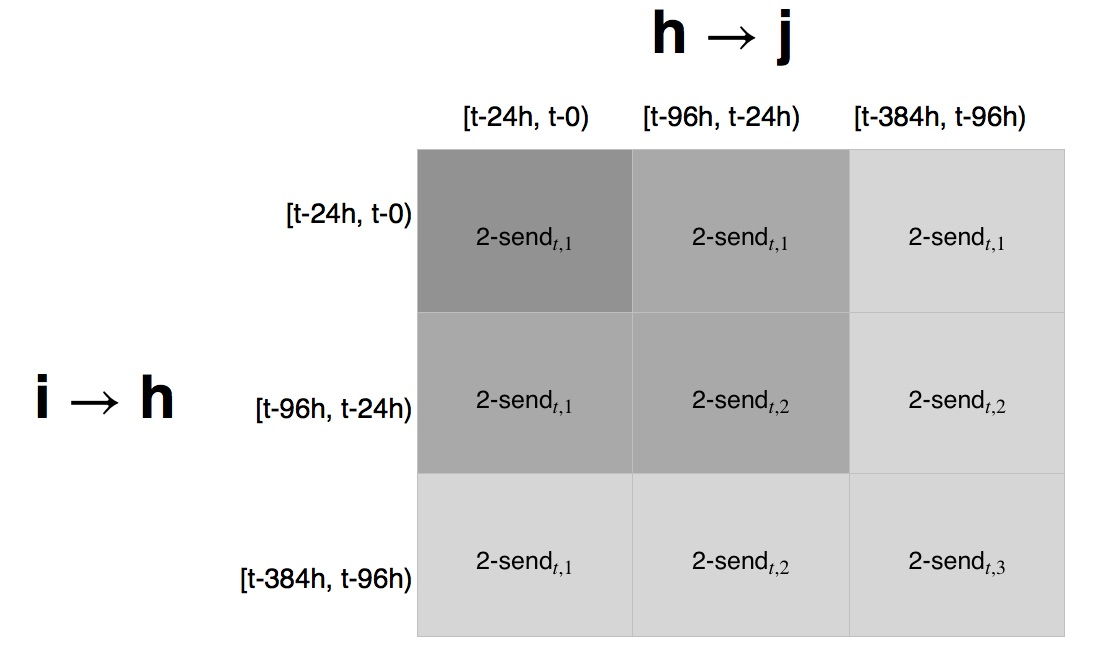
\includegraphics[width=0.49\textwidth]{plots/triadtable.jpg} 
 	\label{fig:triadtable}
 	\caption{2-send defined for each interval $l=1,2,3$. Cells with same shades sum up to one statistic.}
 \end{figure}
 \fi



% In the unusual situation where you want a paper to appear in the
% references without citing it in the main text, use \nocite
%%%%%%%%%%%%%%%%%%%%%%%%%%%%%%%%%%%%%%%%%%%%%%%%%%%%%%%%%%%%%%%%%%%%%%%%%%%%%%%
%%%%%%%%%%%%%%%%%%%%%%%%%%%%%%%%%%%%%%%%%%%%%%%%%%%%%%%%%%%%%%%%%%%%%%%%%%%%%%%
% DELETE THIS PART. DO NOT PLACE CONTENT AFTER THE REFERENCES!
%%%%%%%%%%%%%%%%%%%%%%%%%%%%%%%%%%%%%%%%%%%%%%%%%%%%%%%%%%%%%%%%%%%%%%%%%%%%%%%
%%%%%%%%%%%%%%%%%%%%%%%%%%%%%%%%%%%%%%%%%%%%%%%%%%%%%%%%%%%%%%%%%%%%%%%%%%%%%%%
%%%%%%%%%%%%%%%%%%%%%%%%%%%%%%%%%%%%%%%%%%%%%%%%%%%%%%%%%%%%%%%%%%%%%%%%%%%%%%%
%%%%%%%%%%%%%%%%%%%%%%%%%%%%%%%%%%%%%%%%%%%%%%%%%%%%%%%%%%%%%%%%%%%%%%%%%%%%%%%


\end{document}


% This document was modified from the file originally made available by
% Pat Langley and Andrea Danyluk for ICML-2K. This version was created
% by Iain Murray in 2018. It was modified from a version from Dan Roy in
% 2017, which was based on a version from Lise Getoor and Tobias
% Scheffer, which was slightly modified from the 2010 version by
% Thorsten Joachims & Johannes Fuernkranz, slightly modified from the
% 2009 version by Kiri Wagstaff and Sam Roweis's 2008 version, which is
% slightly modified from Prasad Tadepalli's 2007 version which is a
% lightly changed version of the previous year's version by Andrew
% Moore, which was in turn edited from those of Kristian Kersting and
% Codrina Lauth. Alex Smola contributed to the algorithmic style files.
